% Options for packages loaded elsewhere
\PassOptionsToPackage{unicode}{hyperref}
\PassOptionsToPackage{hyphens}{url}
\PassOptionsToPackage{dvipsnames,svgnames,x11names}{xcolor}
%
\documentclass[
  letterpaper,
  DIV=11,
  numbers=noendperiod]{scrreport}

\usepackage{amsmath,amssymb}
\usepackage{lmodern}
\usepackage{iftex}
\ifPDFTeX
  \usepackage[T1]{fontenc}
  \usepackage[utf8]{inputenc}
  \usepackage{textcomp} % provide euro and other symbols
\else % if luatex or xetex
  \usepackage{unicode-math}
  \defaultfontfeatures{Scale=MatchLowercase}
  \defaultfontfeatures[\rmfamily]{Ligatures=TeX,Scale=1}
\fi
% Use upquote if available, for straight quotes in verbatim environments
\IfFileExists{upquote.sty}{\usepackage{upquote}}{}
\IfFileExists{microtype.sty}{% use microtype if available
  \usepackage[]{microtype}
  \UseMicrotypeSet[protrusion]{basicmath} % disable protrusion for tt fonts
}{}
\makeatletter
\@ifundefined{KOMAClassName}{% if non-KOMA class
  \IfFileExists{parskip.sty}{%
    \usepackage{parskip}
  }{% else
    \setlength{\parindent}{0pt}
    \setlength{\parskip}{6pt plus 2pt minus 1pt}}
}{% if KOMA class
  \KOMAoptions{parskip=half}}
\makeatother
\usepackage{xcolor}
\setlength{\emergencystretch}{3em} % prevent overfull lines
\setcounter{secnumdepth}{5}
% Make \paragraph and \subparagraph free-standing
\ifx\paragraph\undefined\else
  \let\oldparagraph\paragraph
  \renewcommand{\paragraph}[1]{\oldparagraph{#1}\mbox{}}
\fi
\ifx\subparagraph\undefined\else
  \let\oldsubparagraph\subparagraph
  \renewcommand{\subparagraph}[1]{\oldsubparagraph{#1}\mbox{}}
\fi

\usepackage{color}
\usepackage{fancyvrb}
\newcommand{\VerbBar}{|}
\newcommand{\VERB}{\Verb[commandchars=\\\{\}]}
\DefineVerbatimEnvironment{Highlighting}{Verbatim}{commandchars=\\\{\}}
% Add ',fontsize=\small' for more characters per line
\usepackage{framed}
\definecolor{shadecolor}{RGB}{241,243,245}
\newenvironment{Shaded}{\begin{snugshade}}{\end{snugshade}}
\newcommand{\AlertTok}[1]{\textcolor[rgb]{0.68,0.00,0.00}{#1}}
\newcommand{\AnnotationTok}[1]{\textcolor[rgb]{0.37,0.37,0.37}{#1}}
\newcommand{\AttributeTok}[1]{\textcolor[rgb]{0.40,0.45,0.13}{#1}}
\newcommand{\BaseNTok}[1]{\textcolor[rgb]{0.68,0.00,0.00}{#1}}
\newcommand{\BuiltInTok}[1]{\textcolor[rgb]{0.00,0.23,0.31}{#1}}
\newcommand{\CharTok}[1]{\textcolor[rgb]{0.13,0.47,0.30}{#1}}
\newcommand{\CommentTok}[1]{\textcolor[rgb]{0.37,0.37,0.37}{#1}}
\newcommand{\CommentVarTok}[1]{\textcolor[rgb]{0.37,0.37,0.37}{\textit{#1}}}
\newcommand{\ConstantTok}[1]{\textcolor[rgb]{0.56,0.35,0.01}{#1}}
\newcommand{\ControlFlowTok}[1]{\textcolor[rgb]{0.00,0.23,0.31}{#1}}
\newcommand{\DataTypeTok}[1]{\textcolor[rgb]{0.68,0.00,0.00}{#1}}
\newcommand{\DecValTok}[1]{\textcolor[rgb]{0.68,0.00,0.00}{#1}}
\newcommand{\DocumentationTok}[1]{\textcolor[rgb]{0.37,0.37,0.37}{\textit{#1}}}
\newcommand{\ErrorTok}[1]{\textcolor[rgb]{0.68,0.00,0.00}{#1}}
\newcommand{\ExtensionTok}[1]{\textcolor[rgb]{0.00,0.23,0.31}{#1}}
\newcommand{\FloatTok}[1]{\textcolor[rgb]{0.68,0.00,0.00}{#1}}
\newcommand{\FunctionTok}[1]{\textcolor[rgb]{0.28,0.35,0.67}{#1}}
\newcommand{\ImportTok}[1]{\textcolor[rgb]{0.00,0.46,0.62}{#1}}
\newcommand{\InformationTok}[1]{\textcolor[rgb]{0.37,0.37,0.37}{#1}}
\newcommand{\KeywordTok}[1]{\textcolor[rgb]{0.00,0.23,0.31}{#1}}
\newcommand{\NormalTok}[1]{\textcolor[rgb]{0.00,0.23,0.31}{#1}}
\newcommand{\OperatorTok}[1]{\textcolor[rgb]{0.37,0.37,0.37}{#1}}
\newcommand{\OtherTok}[1]{\textcolor[rgb]{0.00,0.23,0.31}{#1}}
\newcommand{\PreprocessorTok}[1]{\textcolor[rgb]{0.68,0.00,0.00}{#1}}
\newcommand{\RegionMarkerTok}[1]{\textcolor[rgb]{0.00,0.23,0.31}{#1}}
\newcommand{\SpecialCharTok}[1]{\textcolor[rgb]{0.37,0.37,0.37}{#1}}
\newcommand{\SpecialStringTok}[1]{\textcolor[rgb]{0.13,0.47,0.30}{#1}}
\newcommand{\StringTok}[1]{\textcolor[rgb]{0.13,0.47,0.30}{#1}}
\newcommand{\VariableTok}[1]{\textcolor[rgb]{0.07,0.07,0.07}{#1}}
\newcommand{\VerbatimStringTok}[1]{\textcolor[rgb]{0.13,0.47,0.30}{#1}}
\newcommand{\WarningTok}[1]{\textcolor[rgb]{0.37,0.37,0.37}{\textit{#1}}}

\providecommand{\tightlist}{%
  \setlength{\itemsep}{0pt}\setlength{\parskip}{0pt}}\usepackage{longtable,booktabs,array}
\usepackage{calc} % for calculating minipage widths
% Correct order of tables after \paragraph or \subparagraph
\usepackage{etoolbox}
\makeatletter
\patchcmd\longtable{\par}{\if@noskipsec\mbox{}\fi\par}{}{}
\makeatother
% Allow footnotes in longtable head/foot
\IfFileExists{footnotehyper.sty}{\usepackage{footnotehyper}}{\usepackage{footnote}}
\makesavenoteenv{longtable}
\usepackage{graphicx}
\makeatletter
\def\maxwidth{\ifdim\Gin@nat@width>\linewidth\linewidth\else\Gin@nat@width\fi}
\def\maxheight{\ifdim\Gin@nat@height>\textheight\textheight\else\Gin@nat@height\fi}
\makeatother
% Scale images if necessary, so that they will not overflow the page
% margins by default, and it is still possible to overwrite the defaults
% using explicit options in \includegraphics[width, height, ...]{}
\setkeys{Gin}{width=\maxwidth,height=\maxheight,keepaspectratio}
% Set default figure placement to htbp
\makeatletter
\def\fps@figure{htbp}
\makeatother

\KOMAoption{captions}{tableheading}
\makeatletter
\makeatother
\makeatletter
\@ifpackageloaded{bookmark}{}{\usepackage{bookmark}}
\makeatother
\makeatletter
\@ifpackageloaded{caption}{}{\usepackage{caption}}
\AtBeginDocument{%
\ifdefined\contentsname
  \renewcommand*\contentsname{Table of contents}
\else
  \newcommand\contentsname{Table of contents}
\fi
\ifdefined\listfigurename
  \renewcommand*\listfigurename{List of Figures}
\else
  \newcommand\listfigurename{List of Figures}
\fi
\ifdefined\listtablename
  \renewcommand*\listtablename{List of Tables}
\else
  \newcommand\listtablename{List of Tables}
\fi
\ifdefined\figurename
  \renewcommand*\figurename{Figure}
\else
  \newcommand\figurename{Figure}
\fi
\ifdefined\tablename
  \renewcommand*\tablename{Table}
\else
  \newcommand\tablename{Table}
\fi
}
\@ifpackageloaded{float}{}{\usepackage{float}}
\floatstyle{ruled}
\@ifundefined{c@chapter}{\newfloat{codelisting}{h}{lop}}{\newfloat{codelisting}{h}{lop}[chapter]}
\floatname{codelisting}{Listing}
\newcommand*\listoflistings{\listof{codelisting}{List of Listings}}
\makeatother
\makeatletter
\@ifpackageloaded{caption}{}{\usepackage{caption}}
\@ifpackageloaded{subcaption}{}{\usepackage{subcaption}}
\makeatother
\makeatletter
\@ifpackageloaded{tcolorbox}{}{\usepackage[many]{tcolorbox}}
\makeatother
\makeatletter
\@ifundefined{shadecolor}{\definecolor{shadecolor}{rgb}{.97, .97, .97}}
\makeatother
\makeatletter
\makeatother
\ifLuaTeX
  \usepackage{selnolig}  % disable illegal ligatures
\fi
\IfFileExists{bookmark.sty}{\usepackage{bookmark}}{\usepackage{hyperref}}
\IfFileExists{xurl.sty}{\usepackage{xurl}}{} % add URL line breaks if available
\urlstyle{same} % disable monospaced font for URLs
\hypersetup{
  pdftitle={Polynomial Regression},
  pdfauthor={Arun \& Zhongyi},
  colorlinks=true,
  linkcolor={blue},
  filecolor={Maroon},
  citecolor={Blue},
  urlcolor={Blue},
  pdfcreator={LaTeX via pandoc}}

\title{Polynomial Regression}
\usepackage{etoolbox}
\makeatletter
\providecommand{\subtitle}[1]{% add subtitle to \maketitle
  \apptocmd{\@title}{\par {\large #1 \par}}{}{}
}
\makeatother
\subtitle{for CDC data with Application for Predicting RSV in USA}
\author{Arun \& Zhongyi}
\date{11/18/2022}

\begin{document}
\maketitle
\ifdefined\Shaded\renewenvironment{Shaded}{\begin{tcolorbox}[borderline west={3pt}{0pt}{shadecolor}, interior hidden, enhanced, boxrule=0pt, sharp corners, frame hidden, breakable]}{\end{tcolorbox}}\fi

\renewcommand*\contentsname{Table of contents}
{
\hypersetup{linkcolor=}
\setcounter{tocdepth}{2}
\tableofcontents
}
\bookmarksetup{startatroot}

\hypertarget{preface}{%
\chapter*{Preface}\label{preface}}
\addcontentsline{toc}{chapter}{Preface}

This is the book to highlight our proposal of new statistical regression
tool, Polynomial Regression Model, to investigate the dynamic of RSV in
USA.

We have seen a dramatic growth of RSV cases this year, but there aren't
any articles founded yet to give prediction of the RSV cases. Based on
the previous researches and the curve of RSV data current analysis has
been carried out.

\bookmarksetup{startatroot}

\hypertarget{introduction}{%
\chapter{Introduction}\label{introduction}}

\textbf{Polynomial Regression for CDC data with Application for
Predicting RSV in USA}

\hypertarget{background}{%
\section{Background}\label{background}}

Respiratory Syncytial Virus (RSV) was discovered in 1956 and has been
recognized as one of the most common causes of childhood illness. RSV
symptoms usually look like a common cold, but it can be serious, leading
to bronchiolitis (inflammation of the small airways in the lung) and
pneumonia, especially for infants and older adults.

According to the Centers for Disease Control and Prevention, RSV results
in around 58,000 annual hospitalizations~and 100 to 300 deaths among
children under 5.\textsuperscript{{[}1{]}} In most regions of the United
States, RSV circulation starts in the fall and peaks in the winter. With
mask-wearing and physical distancing for COVID-19, there were fewer
cases of RSV in 2020. However, RSV cases began to increase in spring
2021 when safety measures relaxed with the arrival of COVID-19 vaccines.
This year, RSV in multiple U.S. regions are nearing seasonal peak
levels. \textsuperscript{{[}2{]}} It is unclear to anyone where RSV will
lead us, a reliable prediction model for RSV data is very crucial for
policymakers to implement fast actions to curb the spread of the
infection, and for public health professionals to understand trends in
virus circulation, estimate disease burden, and respond to outbreaks.

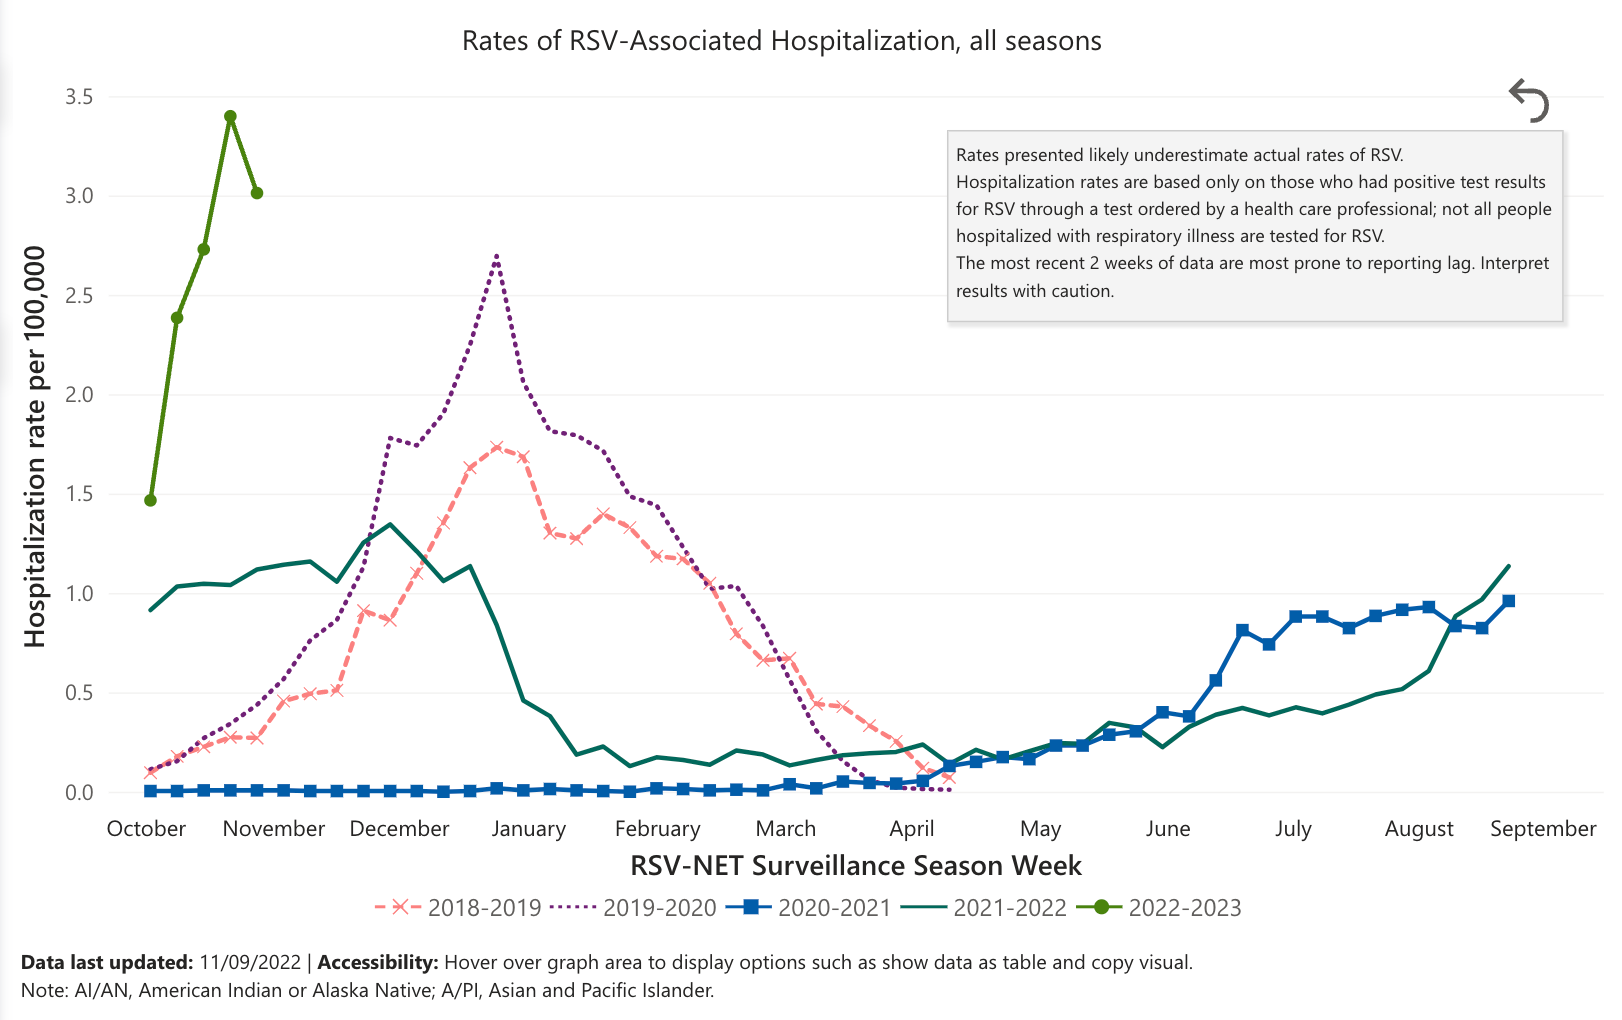
\includegraphics{./images/paste-84838FB2.png}\\

Figure 1.1
\href{https://www.cdc.gov/rsv/research/rsv-net/dashboard.html}{RSV-NET
Interactive Dashboard \textbar{} CDC}

\hypertarget{literature-review}{%
\section{Literature Review}\label{literature-review}}

Respiratory syncytial virus (RSV) infection trend has gained many
researchers' concerns globally. Thongpan, Ilada etc. applied
multivariate time-series analysis to show the possible prediction of RSV
activity based on the climate in Thailand. \textsuperscript{{[}3{]}} The
other researchers tracked RSV through internet search engine data. Oren,
Eyal etc. highlighted the use of search filters and domain adaptation
techniques to assist in identifying spread of both local and more
widespread RSV transmission where comprehensive epidemiological data is
not easy to collect.\textsuperscript{{[}4{]}} Manuel, Britta etc.
applied logistic regression to develop a prediction model and developed
a web-based application to predict the individual probability of RSV
infection.\textsuperscript{{[}5{]}}\\
Furthermore, researchers are using different modeling approaches to
predict the RSV trend. A research done by Reis, Julia etc. tried to
built a real-time RSV prediction system using a
susceptible-infectious-recovered (SIR) model in conjunction with an
ensemble adjustment Kalman filter (EAKF) and 10 years CDC
data\textsuperscript{{[}6{]}}. Bayesian stochastic
susceptible‐infected‐recovered‐susceptible (SIRS) model was presented by
Corberán-Vallet etc. to understand RSV dynamics in the region of
Valencia, Spain. However, this continuous‐time deterministic model is
not suitable when the initial number of infected individuals is
small\textsuperscript{{[}7{]}}. Leecaster, Molly etc. use simple linear
regression to explore the relationship between three epidemic
characteristics (final epidemic size, days to peak, and epidemic length)
and exponential growth calculated from four weeks of daily case data.
They find out exponential growth was correlated to epidemic
characteristics\textsuperscript{{[}8{]}}.

\hypertarget{problem-statement}{%
\section{Problem Statement}\label{problem-statement}}

We have seen a dramatic growth of RSV cases this year, but there are not
any articles founded yet to give prediction of the RSV cases now. Based
on the previous researches and the curve of RSV data, we propose a new
statistical regression tool---\textbf{Polynomial Regression Model} ---
to investigate the dynamics of RSV in USA.

\bookmarksetup{startatroot}

\hypertarget{methodology}{%
\chapter{Methodology}\label{methodology}}

The data set for this research is from **RSV Hospitalization
Surveillance Network (RSV-NET)** (one of CDC research and surveillance
platforms) ,which conducts population-based surveillance system for
laboratory-confirmed COVID-19, RSV, and influenza-associated
hospitalizations in the US among children younger than 18 years of age
and adults.\textsuperscript{{[}8{]}}

RSV-NET has been collecting RSV-associated hospitalizations in adults
and children since 2018-2019 season from 58 counties in 12 states,
including California, Colorado, Connecticut, Georgia, Maryland,
Michigan, Minnesota, New Mexico, New York, Oregon, Tennessee, and Utah.
Almost 9\% of the U.S. population is covered and reported by the
RSV-NET.

\hypertarget{about-this-dataset}{%
\section{About this Dataset}\label{about-this-dataset}}

\begin{enumerate}
\def\labelenumi{\arabic{enumi}.}
\item
  \textbf{Time frame:} In season 2018-2019, 2019-2020, data collected is
  from October 1 to April 30. In season 2020-2021, 2021-2022, 2022-2023,
  data collected is from October 1 to October 1 next year.
\item
  \textbf{How an entry is made in data set:}

  A case is defined by laboratory-confirmed RSV in a person who Lives in
  a defined RSV-NET surveillance area AND Tests positive for RSV within
  14 days before or during hospitalization. Evidence of RSV infection
  can be obtained through several laboratory tests.
\item
  \textbf{Variables:}

  In the original data set, it has 8 columns which are described in
  below table

  \begin{longtable}[]{@{}
    >{\raggedright\arraybackslash}p{(\columnwidth - 2\tabcolsep) * \real{0.0462}}
    >{\raggedright\arraybackslash}p{(\columnwidth - 2\tabcolsep) * \real{0.9538}}@{}}
  \toprule()
  \begin{minipage}[b]{\linewidth}\raggedright
  Column Name
  \end{minipage} & \begin{minipage}[b]{\linewidth}\raggedright
  Description
  \end{minipage} \\
  \midrule()
  \endhead
  State & Represents the state name from which data was collected.
  Entire state means all 9 states considered in this dataset. \\
  MMWR Year & Represents Year \\
  \textbf{MMWR Week} & Represents week of that year. MMWR -
  \emph{Morbidity and Mortality Weekly Report,} is prepared by the
  Centers for Disease Control and Prevention (CDC). \\
  Season & As the data is collected between October to April, this
  represents the duration of the year. \\
  Age Category & Age limit \\
  Sex & Male/Female \\
  Race & Black, White, American Indian/Alaska Native and Asian/Pacific
  Islander people are categorized as non-Hispanic. Hispanic people could
  be of any race. If Hispanic ethnicity was unknown, non-Hispanic
  ethnicity was assumed. \\
  \textbf{Rate} & calculated as the number of residents in a
  surveillance area who are hospitalized with laboratory-confirmed RSV
  divided by the total population estimate for that area. {[}NCHS
  bridged-race
  population{]}(\url{https://www.cdc.gov/nchs/nvss/bridged_race.htm})~estimates
  are used as denominators for rate calculations. \\
  \bottomrule()
  \end{longtable}

  The data was last updated on \textbf{17th November 2022}. We have
  considered two sets of data, one with last 12 months of YTD data and
  another one with 24 months of YTD data for our calculations.
\end{enumerate}

\hypertarget{methods}{%
\section{Methods}\label{methods}}

\hypertarget{why-polynomial-regression}{%
\subsection{\texorpdfstring{\emph{Why Polynomial
Regression?}}{Why Polynomial Regression?}}\label{why-polynomial-regression}}

In simple linear regression algorithm only works when the relationship
between the data is linear, suppose if we have non-linear data then
linear regression will not be capable to draw a best-fit line and it
fails in such conditions. Consider the below diagram which has a
non-linear relationship and you can see the Linear regression results on
it, which does not perform well and doesn't come close to reality.
Hence, we introduce polynomial regression to overcome this problem,
which helps identify the curvilinear relationship between independent
and dependent variables.

\includegraphics{./images/1_7w8mfB_Ecfr0x76Vc7qang.gif}

\hypertarget{how-polynomial-regression-overcomes-the-problem-of-non-linear-data}{%
\subsection{\texorpdfstring{\textbf{How Polynomial Regression Overcomes
the problem of Non-Linear
data?}}{How Polynomial Regression Overcomes the problem of Non-Linear data?}}\label{how-polynomial-regression-overcomes-the-problem-of-non-linear-data}}

\includegraphics{./images/PolyRegressionConversion.gif}

Polynomial regression is a form of Linear regression where only due to
the Non-linear relationship between dependent and independent variables
we add some polynomial terms to linear regression to convert it into
Polynomial regression.

Suppose we have X as Independent data and Y as dependent data. Before
feeding data to a mode in preprocessing stage we convert the input
variables into polynomial terms using some degree.

Consider an example my input value is 35 and the degree of a polynomial
is 2 so I will find 35 power 0, 35 power 1, and 35 power 2 And this
helps to interpret the non-linear relationship in data.\\
The equation of polynomial becomes something like
this.\textsuperscript{{[}9{]}}

\textbf{y = 𝛽\textsubscript{0} + 𝛽\textsubscript{1}x\textsubscript{1} +
𝛽\textsubscript{2}x\textsubscript{1}\textsuperscript{2} + \ldots{} +
𝛽\textsubscript{n}x\textsubscript{1}\textsuperscript{n}}

The degree of order which to use is a Hyper-parameter, and we need to
choose it wisely. But using a high degree of polynomial tries to
over-fit the data and for smaller values of degree, the model tries to
under-fit so we need to find the optimum value of a degree.

If you see the equation of polynomial regression carefully, then we can
see that we are trying to estimate the relationship between coefficients
and y. And the values of x and y are already given to us, only we need
to determine coefficients and the degree of coefficient here is 1 only,
and degree one represents simple linear regression Hence, Polynomial
regression is also known as polynomial Linear regression.

\includegraphics{./images/polynomial_regression_fit.gif}

In~statistics,~\textbf{polynomial regression}~is a form of~regression
analysis~in which the relationship between the~independent
variable~\emph{x}~and the~dependent variable~\emph{y}~is modelled as
an~\emph{n}th degree~polynomial~in~\emph{x}. Polynomial regression fits
a nonlinear relationship between the value of~\emph{x}~and the
corresponding~conditional mean~of~\emph{y}, denoted
E(\emph{y}~\textbar{}\emph{x}). Although~\emph{polynomial
regression}~fits a nonlinear model to the data, as a~statistical
estimation~problem it is linear, in the sense that the regression
function E(\emph{y}~\textbar~\emph{x}) is linear in the
unknown~parameters~that are estimated from the~data. For this reason,
polynomial regression is considered to be a special case of~multiple
linear regression. The explanatory (independent) variables resulting
from the polynomial expansion of the ``baseline'' variables are known as
higher-degree terms. Such variables are also used
in~classification~settings\textsuperscript{{[}10{]}}.

\bookmarksetup{startatroot}

\hypertarget{data-analysis-and-results}{%
\chapter{Data Analysis and Results}\label{data-analysis-and-results}}

In this part, a model to predict RSV hospitalization rate is trying to
be established. The question is what range of data we should be included
to better predict the RSV rate, one year, or two year. This question
will be solved in this part.

Before that, the data distribution of RSV hospitalization rates from
2018 to now is displayed below.

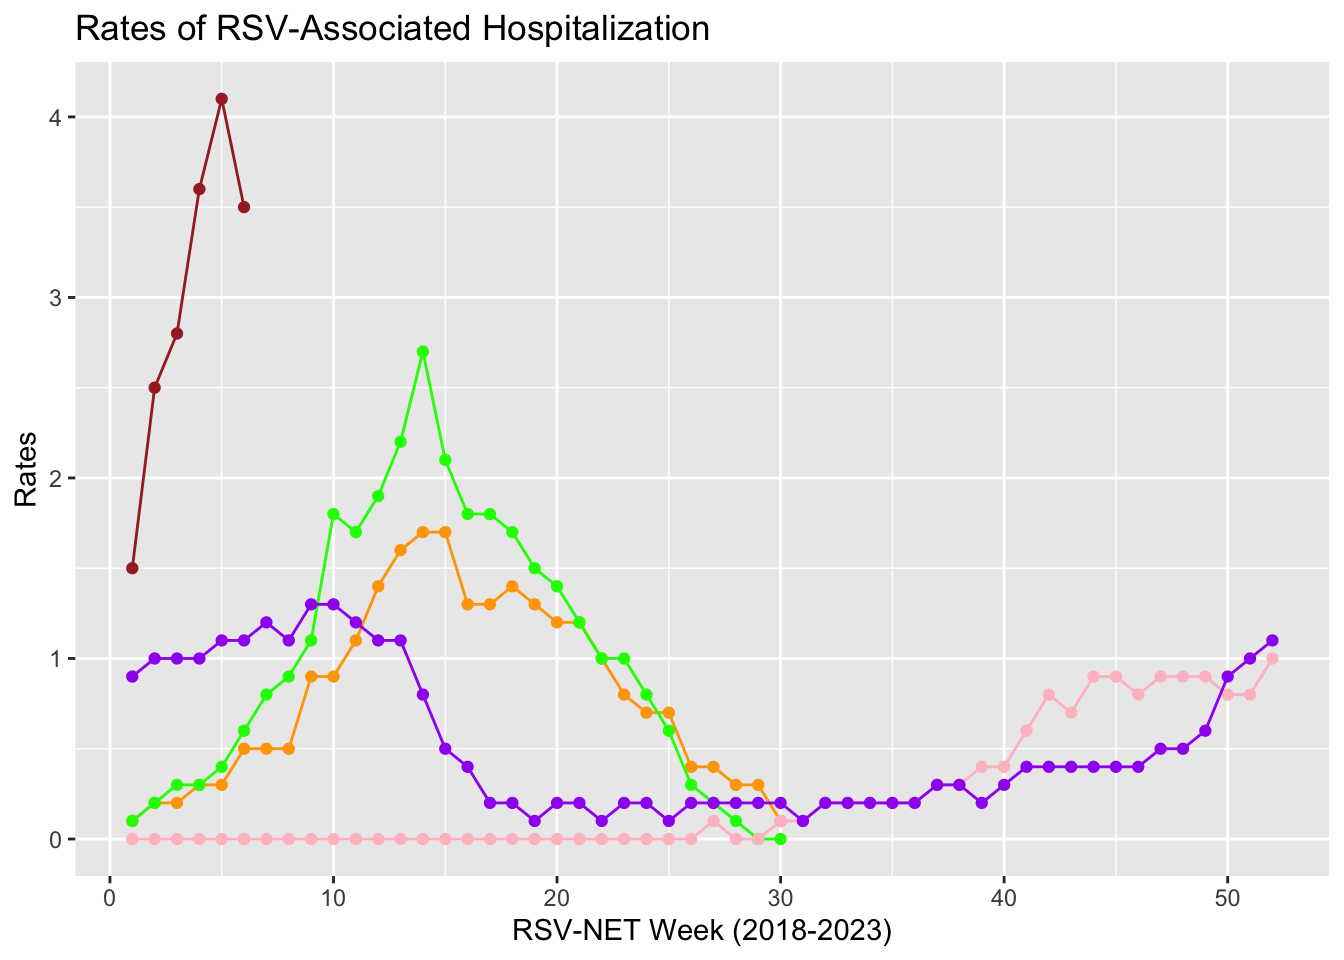
\includegraphics{./RSVNET-data-analysis-and-results_files/figure-pdf/unnamed-chunk-1-1.pdf}

\textbf{\emph{Note: (1) color orange: year 2018-2019; color green: year
2019-2020; color pink: year 2020-2021; color purple: 2021-2022; color
brown: 2022-2023}}

\textbf{\emph{(2)In 2018-2020, data shown is from October 1 to April 30
each year; In 2020-now, data is from October 1 to the next year October
1 each year.}}

\textbf{\emph{(3)In year 2020-2021, because of Covid restriction and
mask mandate, there are fewer cases.}}

From the graph below, we notice that data is not linear distributed, and
curved lines are noticed. So, polynomial regression is selected to be
our approach.

\hypertarget{one-year-to-date-data-analysis}{%
\section{One year-to-date data
Analysis}\label{one-year-to-date-data-analysis}}

A model built for 1 year-to date data follows the following steps.

\hypertarget{data-pre-processing-and-distribution}{%
\subsection{Data Pre-processing and
Distribution}\label{data-pre-processing-and-distribution}}

Data was examined before our modeling, including checking for missing
values and removing outlines.

\begin{verbatim}
         Week oneyeartodate 
            0             0 
\end{verbatim}

One-year-to-date data distribution with a curve line was shown below. We
can see that the straight line is unable to capture the patterns in the
data. Data is being under-fitting.

\begin{Shaded}
\begin{Highlighting}[]
\FunctionTok{ggplot}\NormalTok{(data1,}\FunctionTok{aes}\NormalTok{(}\AttributeTok{x=}\NormalTok{Week,}\AttributeTok{y=}\NormalTok{oneyeartodate))}\SpecialCharTok{+}\FunctionTok{geom\_point}\NormalTok{(}\AttributeTok{data=}\NormalTok{data1,}\FunctionTok{aes}\NormalTok{(}\AttributeTok{x=}\NormalTok{Week,}\AttributeTok{y=}\NormalTok{oneyeartodate),}\AttributeTok{color=}\StringTok{"blue"}\NormalTok{)}\SpecialCharTok{+}\FunctionTok{stat\_smooth}\NormalTok{(}\AttributeTok{method=}\NormalTok{lm,}\AttributeTok{formula=}\NormalTok{y}\SpecialCharTok{\textasciitilde{}}\FunctionTok{poly}\NormalTok{(x,}\DecValTok{1}\NormalTok{,}\AttributeTok{raw=}\ConstantTok{TRUE}\NormalTok{))}\SpecialCharTok{+}
  \FunctionTok{labs}\NormalTok{(}\AttributeTok{x=}\StringTok{"RSV{-}NET week Week 46th,2021{-}Week 45th,2022"}\NormalTok{,}\AttributeTok{y=}\StringTok{"Rates"}\NormalTok{,}\AttributeTok{title=}\StringTok{"Rates of RSV{-}Associated Hospitalization One year{-}to{-}date"}\NormalTok{)}
\end{Highlighting}
\end{Shaded}

\begin{figure}[H]

{\centering 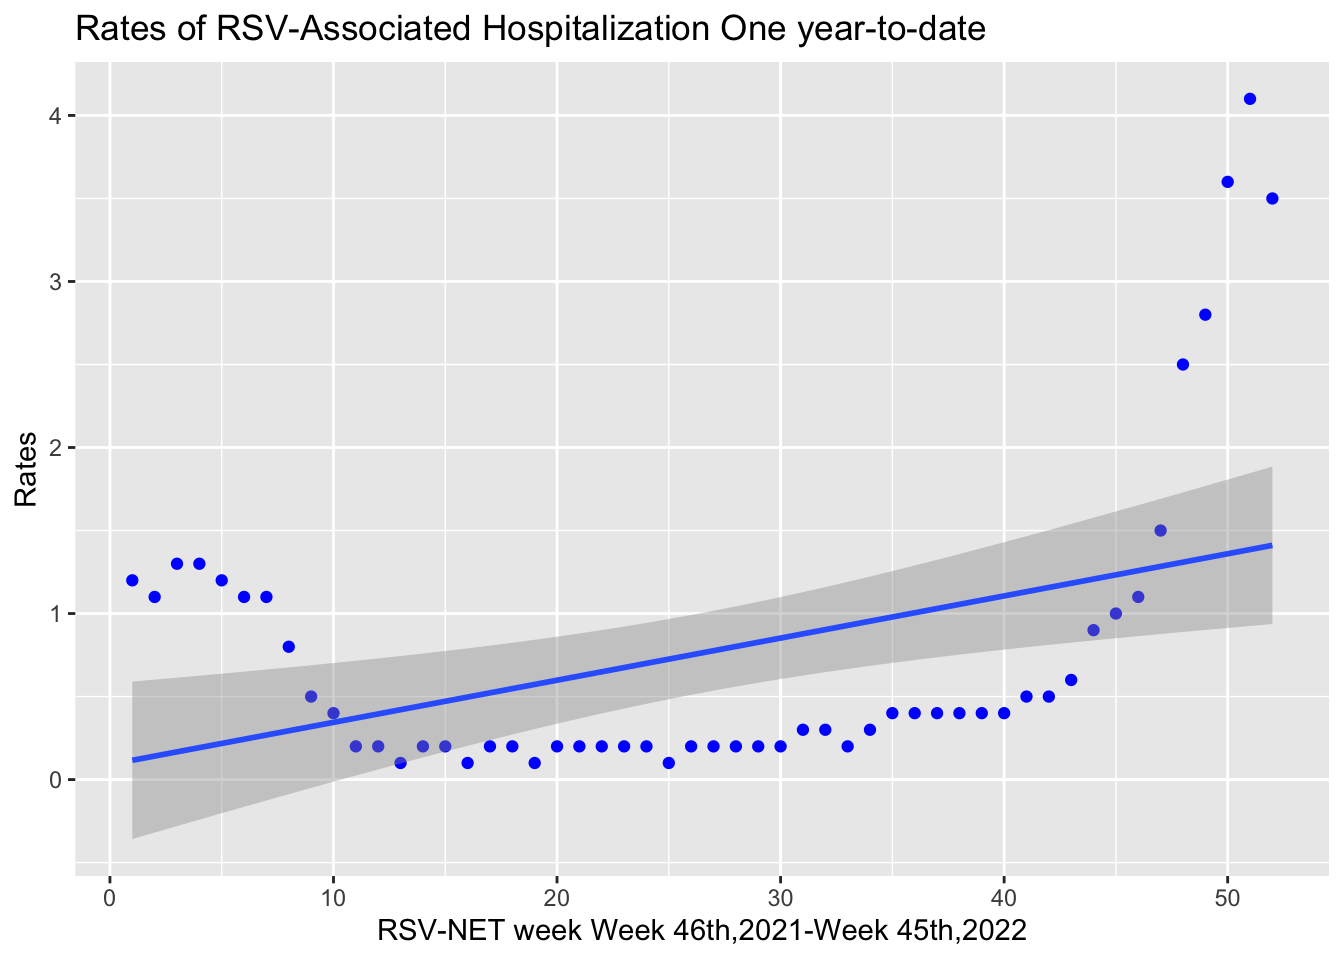
\includegraphics{./RSVNET-data-analysis-and-results_files/figure-pdf/unnamed-chunk-3-1.pdf}

}

\end{figure}

\hypertarget{polynomial-regression-and-results}{%
\subsection{Polynomial Regression and
results}\label{polynomial-regression-and-results}}

To overcome under-fitting, we generate a higher order equation to
increase the complexity of the model. To do that, we add powers of the
original features as new features through polynomial regression
analysis. Data was split into train data and test data, and a comparison
was made to decide which degree of model is the best fit for the data
from Nov 2021 to Nov 2022.

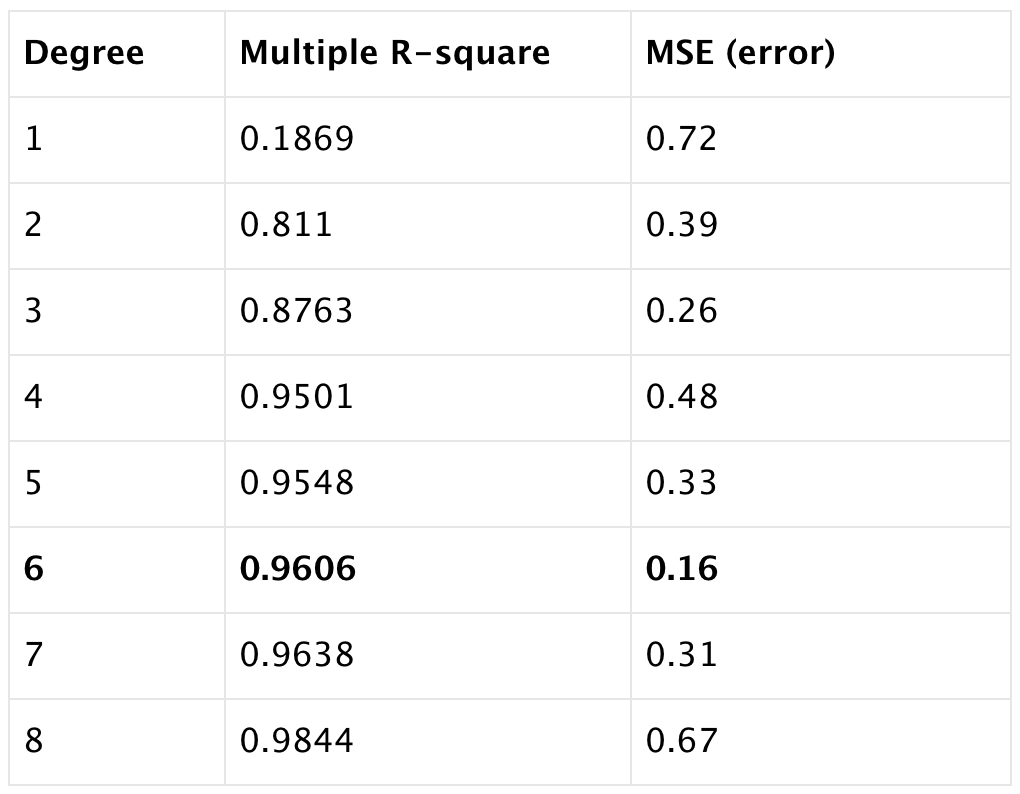
\includegraphics[width=5.98958in,height=\textheight]{./images/paste-99DEEB9C.png}

\begin{Shaded}
\begin{Highlighting}[]
\NormalTok{my\_data}\OtherTok{\textless{}{-}}\NormalTok{data1}

\CommentTok{\#split data into training and test}

\FunctionTok{set.seed}\NormalTok{(}\DecValTok{150}\NormalTok{)}

\NormalTok{training.samples }\OtherTok{\textless{}{-}}\NormalTok{data1}\SpecialCharTok{$}\NormalTok{oneyeartodate }\SpecialCharTok{\%\textgreater{}\%}

  \FunctionTok{createDataPartition}\NormalTok{(}\AttributeTok{p=}\FloatTok{0.8}\NormalTok{,}\AttributeTok{list=}\ConstantTok{FALSE}\NormalTok{)}

\NormalTok{train.data}\OtherTok{\textless{}{-}}\NormalTok{my\_data[training.samples, ]}

\NormalTok{test.data}\OtherTok{\textless{}{-}}\NormalTok{my\_data[}\SpecialCharTok{{-}}\NormalTok{training.samples, ]}

\CommentTok{\#build model}

\NormalTok{model}\OtherTok{\textless{}{-}}\FunctionTok{lm}\NormalTok{(oneyeartodate}\SpecialCharTok{\textasciitilde{}}\FunctionTok{poly}\NormalTok{(Week,}\DecValTok{6}\NormalTok{,}\AttributeTok{raw=}\ConstantTok{TRUE}\NormalTok{),}\AttributeTok{data=}\NormalTok{train.data)}

\FunctionTok{summary}\NormalTok{(model)}
\end{Highlighting}
\end{Shaded}

\begin{verbatim}

Call:
lm(formula = oneyeartodate ~ poly(Week, 6, raw = TRUE), data = train.data)

Residuals:
     Min       1Q   Median       3Q      Max 
-0.64803 -0.09377  0.00132  0.10147  0.53149 

Coefficients:
                             Estimate Std. Error t value Pr(>|t|)  
(Intercept)                 9.166e-01  6.768e-01   1.354   0.1843  
poly(Week, 6, raw = TRUE)1  3.117e-01  2.695e-01   1.157   0.2553  
poly(Week, 6, raw = TRUE)2 -7.364e-02  3.657e-02  -2.014   0.0518 .
poly(Week, 6, raw = TRUE)3  5.399e-03  2.292e-03   2.356   0.0242 *
poly(Week, 6, raw = TRUE)4 -1.781e-04  7.255e-05  -2.455   0.0192 *
poly(Week, 6, raw = TRUE)5  2.714e-06  1.126e-06   2.411   0.0213 *
poly(Week, 6, raw = TRUE)6 -1.530e-08  6.796e-09  -2.252   0.0307 *
---
Signif. codes:  0 '***' 0.001 '**' 0.01 '*' 0.05 '.' 0.1 ' ' 1

Residual standard error: 0.2112 on 35 degrees of freedom
Multiple R-squared:  0.9606,    Adjusted R-squared:  0.9538 
F-statistic:   142 on 6 and 35 DF,  p-value: < 2.2e-16
\end{verbatim}

\begin{Shaded}
\begin{Highlighting}[]
\CommentTok{\#predict using the model}

\NormalTok{predictions}\OtherTok{\textless{}{-}}\NormalTok{model }\SpecialCharTok{\%\textgreater{}\%} \FunctionTok{predict}\NormalTok{(test.data)}

\CommentTok{\#error}

\NormalTok{error}\OtherTok{\textless{}{-}}\FunctionTok{RMSE}\NormalTok{(predictions,test.data}\SpecialCharTok{$}\NormalTok{oneyeartodate)}
\end{Highlighting}
\end{Shaded}

We listed the Multiple R-squared and root mean square error (RMSE, or
error) when the degree of polynomials from 1 to 10. We can observe with
the increase of the degree, multiple r-square increase too. While error
goes down and then goes up again when we keep adding the powers of the
original features. That incease of the error is caused by data
overfitting, the model try to pass through most of the data points.

The best model we looking for is the one with high multiple R square
(0.9606) and low RMSE (0.16), so we select the model with degree of 6.

\hypertarget{two-year-to-date-data-analysis}{%
\section{Two year-to-date data
Analysis}\label{two-year-to-date-data-analysis}}

We also analysis the date from Nov, 2020 to Nov, 2022 following the same
steps, and try to see if including more data points will get a better
prediction model.

\hypertarget{data-pre-processing-and-distribution-1}{%
\subsection{Data Pre-processing and
Distribution}\label{data-pre-processing-and-distribution-1}}

Two-year-to-date data distribution with a curve line was shown below.
Data is under fitted, polynomial regression is needed to increase the
complexity of the model.

\begin{verbatim}
         Week twoyeartodate 
            0             0 
\end{verbatim}

\begin{Shaded}
\begin{Highlighting}[]
\FunctionTok{ggplot}\NormalTok{(data2,}\FunctionTok{aes}\NormalTok{(}\AttributeTok{x=}\NormalTok{Week,}\AttributeTok{y=}\NormalTok{twoyeartodate))}\SpecialCharTok{+}\FunctionTok{geom\_point}\NormalTok{(}\AttributeTok{data=}\NormalTok{data2,}\FunctionTok{aes}\NormalTok{(}\AttributeTok{x=}\NormalTok{Week,}\AttributeTok{y=}\NormalTok{twoyeartodate),}\AttributeTok{color=}\StringTok{"purple"}\NormalTok{)}\SpecialCharTok{+}\FunctionTok{stat\_smooth}\NormalTok{(}\AttributeTok{method=}\NormalTok{lm,}\AttributeTok{formula=}\NormalTok{y}\SpecialCharTok{\textasciitilde{}}\FunctionTok{poly}\NormalTok{(x,}\DecValTok{1}\NormalTok{,}\AttributeTok{raw=}\ConstantTok{TRUE}\NormalTok{))}\SpecialCharTok{+}
  \FunctionTok{labs}\NormalTok{(}\AttributeTok{x=}\StringTok{"RSV{-}NET week Week 46th,2020{-}Week 45th,2022"}\NormalTok{,}\AttributeTok{y=}\StringTok{"Rates"}\NormalTok{,}\AttributeTok{title=}\StringTok{"Rates of RSV{-}Associated Hospitalization two year{-}to{-}date"}\NormalTok{)}
\end{Highlighting}
\end{Shaded}

\begin{figure}[H]

{\centering 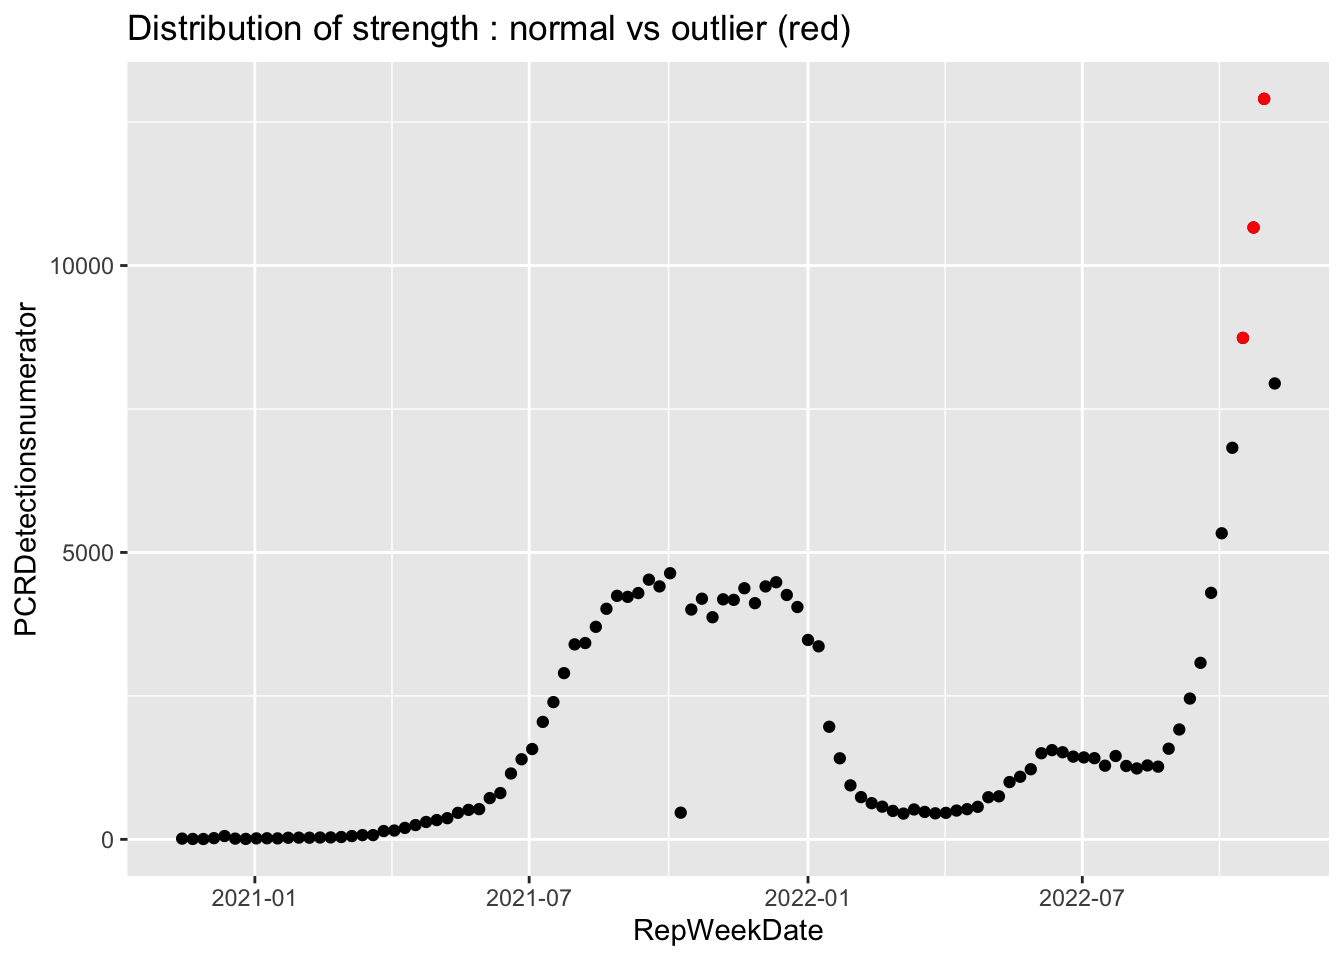
\includegraphics{./RSVNET-data-analysis-and-results_files/figure-pdf/unnamed-chunk-6-1.pdf}

}

\end{figure}

\hypertarget{polynomial-regression-and-results-1}{%
\subsection{Polynomial Regression and
results}\label{polynomial-regression-and-results-1}}

The best model for the most recent two year data we select is at the
degree of 5 with multiple r-square 0.92 and error 0.24.

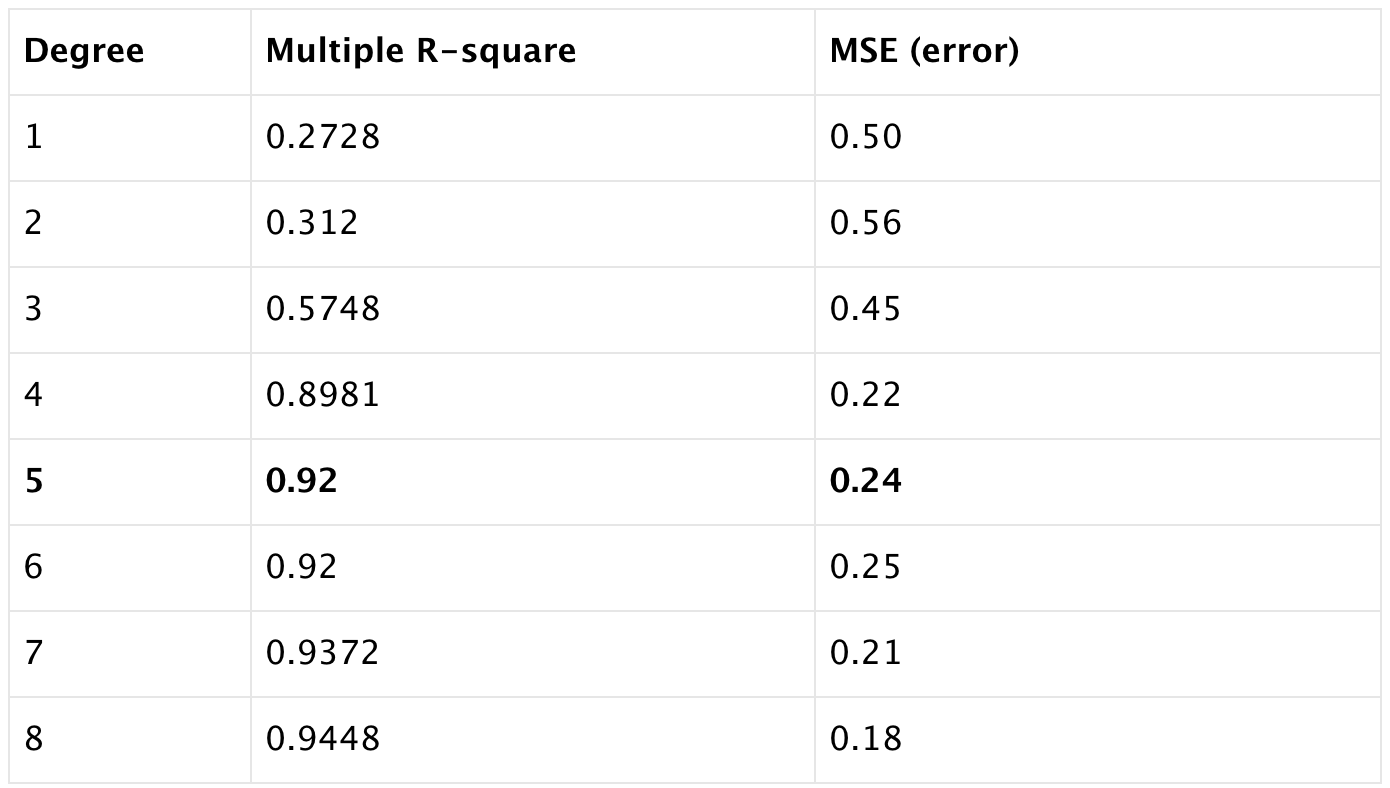
\includegraphics[width=6.17708in,height=\textheight]{./images/paste-9BB97AC3.png}

\begin{Shaded}
\begin{Highlighting}[]
\NormalTok{my\_data2}\OtherTok{\textless{}{-}}\NormalTok{data2}

\CommentTok{\#split data into training and test}

\FunctionTok{set.seed}\NormalTok{(}\DecValTok{150}\NormalTok{)}

\NormalTok{training.samples }\OtherTok{\textless{}{-}}\NormalTok{data2}\SpecialCharTok{$}\NormalTok{twoyeartodate }\SpecialCharTok{\%\textgreater{}\%}

  \FunctionTok{createDataPartition}\NormalTok{(}\AttributeTok{p=}\FloatTok{0.8}\NormalTok{,}\AttributeTok{list=}\ConstantTok{FALSE}\NormalTok{)}

\NormalTok{train.data2}\OtherTok{\textless{}{-}}\NormalTok{my\_data2[training.samples, ]}

\NormalTok{test.data2}\OtherTok{\textless{}{-}}\NormalTok{my\_data2[}\SpecialCharTok{{-}}\NormalTok{training.samples, ]}

\CommentTok{\#build model}

\NormalTok{model2}\OtherTok{\textless{}{-}}\FunctionTok{lm}\NormalTok{(twoyeartodate}\SpecialCharTok{\textasciitilde{}}\FunctionTok{poly}\NormalTok{(Week,}\DecValTok{5}\NormalTok{,}\AttributeTok{raw=}\ConstantTok{TRUE}\NormalTok{),}\AttributeTok{data=}\NormalTok{train.data2)}

\FunctionTok{summary}\NormalTok{(model2)}
\end{Highlighting}
\end{Shaded}

\begin{verbatim}

Call:
lm(formula = twoyeartodate ~ poly(Week, 5, raw = TRUE), data = train.data2)

Residuals:
    Min      1Q  Median      3Q     Max 
-0.5665 -0.1158  0.0259  0.1323  0.6496 

Coefficients:
                             Estimate Std. Error t value Pr(>|t|)    
(Intercept)                 1.069e-01  1.526e-01   0.700  0.48573    
poly(Week, 5, raw = TRUE)1 -2.892e-02  2.961e-02  -0.977  0.33156    
poly(Week, 5, raw = TRUE)2  8.463e-04  1.752e-03   0.483  0.63048    
poly(Week, 5, raw = TRUE)3  4.486e-05  4.235e-05   1.059  0.29274    
poly(Week, 5, raw = TRUE)4 -1.265e-06  4.444e-07  -2.846  0.00565 ** 
poly(Week, 5, raw = TRUE)5  7.821e-09  1.683e-09   4.646 1.33e-05 ***
---
Signif. codes:  0 '***' 0.001 '**' 0.01 '*' 0.05 '.' 0.1 ' ' 1

Residual standard error: 0.2338 on 79 degrees of freedom
Multiple R-squared:   0.92, Adjusted R-squared:  0.9149 
F-statistic: 181.6 on 5 and 79 DF,  p-value: < 2.2e-16
\end{verbatim}

\begin{Shaded}
\begin{Highlighting}[]
\CommentTok{\#predict using the model}

\NormalTok{predictions2}\OtherTok{\textless{}{-}}\NormalTok{model2 }\SpecialCharTok{\%\textgreater{}\%} \FunctionTok{predict}\NormalTok{(test.data2)}

\CommentTok{\#error}

\NormalTok{error}\OtherTok{\textless{}{-}}\FunctionTok{RMSE}\NormalTok{(predictions2,test.data2}\SpecialCharTok{$}\NormalTok{twoyeartodate)}
\end{Highlighting}
\end{Shaded}

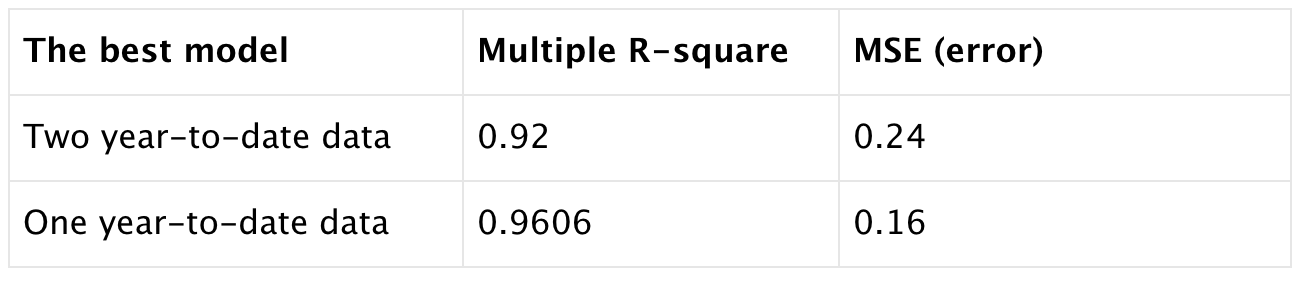
\includegraphics[width=5.875in,height=\textheight]{./images/paste-09152757.png}

By comparison the two year-to-date data with the one year-to-date data,
it shows that building RSV hospitalization rate model containing most
recent one year data create the best prediction model.

\hypertarget{model-performance}{%
\section{Model performance}\label{model-performance}}

The model for RSV hospitalization rate from Nov, 2021 to Nov, 2022 was
formed as:

\textbf{RSV Hospitalization Rate = 0.917 + 0.312Week -
0.074Week\textsuperscript{2} + 0.0054Week\textsuperscript{3} -
0.00018Week\textsuperscript{4} + 0.0000027Week\textsuperscript{5} -
0.000000015Week\textsuperscript{6}}

\begin{verbatim}
                                Estimate   Std. Error   t value   Pr(>|t|)
(Intercept)                 9.165688e-01 6.768202e-01  1.354228 0.18434303
poly(Week, 6, raw = TRUE)1  3.116708e-01 2.694685e-01  1.156613 0.25526403
poly(Week, 6, raw = TRUE)2 -7.363560e-02 3.656703e-02 -2.013716 0.05177789
poly(Week, 6, raw = TRUE)3  5.399174e-03 2.292002e-03  2.355659 0.02422194
poly(Week, 6, raw = TRUE)4 -1.781037e-04 7.255321e-05 -2.454801 0.01921034
poly(Week, 6, raw = TRUE)5  2.713662e-06 1.125680e-06  2.410688 0.02131056
poly(Week, 6, raw = TRUE)6 -1.530307e-08 6.795953e-09 -2.251792 0.03071366
\end{verbatim}

When we compare the actual hospitalization with the predicted value from
our model, we can get the numbers as follow. We can conclude that the
model created is a good fit. It also can be shown at the graph below.

\begin{Shaded}
\begin{Highlighting}[]
\NormalTok{compare }\OtherTok{\textless{}{-}}\FunctionTok{data.frame}\NormalTok{(}\AttributeTok{actual=}\NormalTok{test.data}\SpecialCharTok{$}\NormalTok{oneyeartodate,}\AttributeTok{predicted=}\NormalTok{predictions)}
\FunctionTok{head}\NormalTok{(compare,}\AttributeTok{n=}\DecValTok{10}\NormalTok{)}
\end{Highlighting}
\end{Shaded}

\begin{verbatim}
   actual  predicted
1     1.2 1.15982773
2     1.1 1.28579756
3     0.5 0.67668810
4     0.2 0.42365176
5     0.1 0.07749228
6     0.2 0.12270299
7     0.2 0.18344956
8     0.3 0.27587346
9     0.3 0.24948406
10    2.5 2.16341891
\end{verbatim}

\begin{Shaded}
\begin{Highlighting}[]
\NormalTok{modelPerformance}\OtherTok{=}\FunctionTok{data.frame}\NormalTok{(}\AttributeTok{RMSE=}\FunctionTok{RMSE}\NormalTok{(predictions,test.data}\SpecialCharTok{$}\NormalTok{oneyeartodate),}\AttributeTok{R2=}\FunctionTok{R2}\NormalTok{(predictions,test.data}\SpecialCharTok{$}\NormalTok{oneyeartodate))}
\FunctionTok{ggplot}\NormalTok{(train.data,}\FunctionTok{aes}\NormalTok{(Week,oneyeartodate))}\SpecialCharTok{+}\FunctionTok{geom\_point}\NormalTok{()}\SpecialCharTok{+}\FunctionTok{stat\_smooth}\NormalTok{(}\AttributeTok{method=}\NormalTok{lm,}\AttributeTok{formula=}\NormalTok{y}\SpecialCharTok{\textasciitilde{}}\FunctionTok{poly}\NormalTok{(x,}\DecValTok{6}\NormalTok{,}\AttributeTok{raw=}\ConstantTok{TRUE}\NormalTok{))}
\end{Highlighting}
\end{Shaded}

\begin{figure}[H]

{\centering 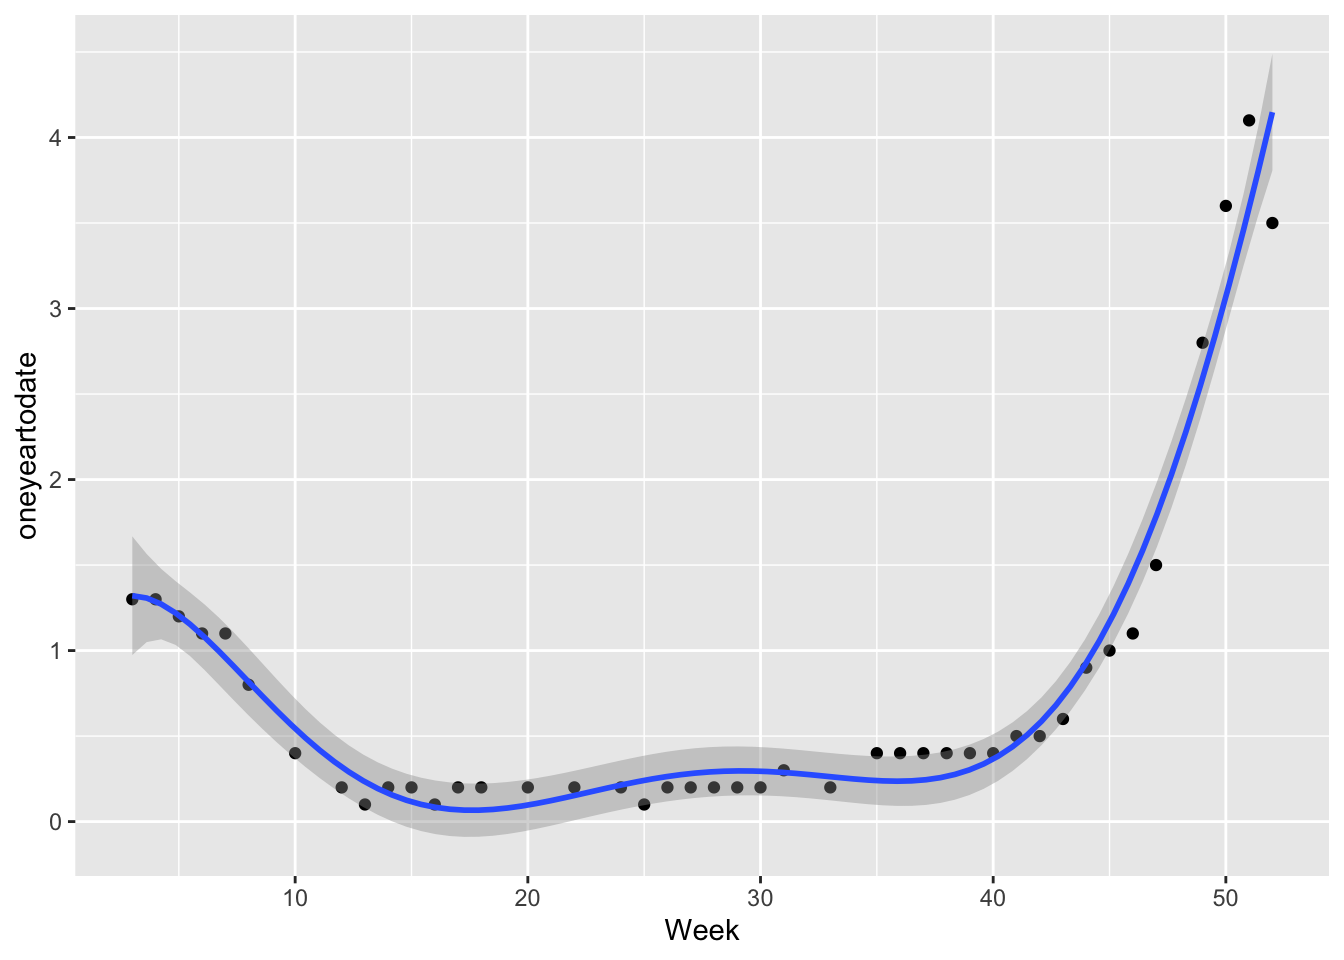
\includegraphics{./RSVNET-data-analysis-and-results_files/figure-pdf/unnamed-chunk-10-1.pdf}

}

\end{figure}

\hypertarget{predict-the-future-value}{%
\section{Predict the future value}\label{predict-the-future-value}}

We have got our model with the equation for the RSV hospitalization rate
data in the recent one year: \textbf{RSV Hospitalization Rate = 0.917 +
0.312Week - 0.074Week\textsuperscript{2} + 0.0054Week\textsuperscript{3}
- 0.00018Week\textsuperscript{4} + 0.0000027Week\textsuperscript{5} -
0.000000015Week\textsuperscript{6}}

On the ground of this model, we predicted the future RSV hospitalization
rates in the next three months. A table is listed below to show the
trend. Following the trend in our model, rates keep going up and a rate
of 9 could be reached at the beginning of next year.

\begin{Shaded}
\begin{Highlighting}[]
\NormalTok{newcases }\OtherTok{\textless{}{-}} \FunctionTok{data.frame}\NormalTok{(}\AttributeTok{Week =} \FunctionTok{c}\NormalTok{(}\DecValTok{53}\NormalTok{,}\DecValTok{54}\NormalTok{,}\DecValTok{55}\NormalTok{,}\DecValTok{56}\NormalTok{,}\DecValTok{57}\NormalTok{,}\DecValTok{58}\NormalTok{,}\DecValTok{59}\NormalTok{,}\DecValTok{60}\NormalTok{,}\DecValTok{61}\NormalTok{,}\DecValTok{62}\NormalTok{,}\DecValTok{63}\NormalTok{,}\DecValTok{64}\NormalTok{))}
\FunctionTok{predict}\NormalTok{(model,newcases)}
\end{Highlighting}
\end{Shaded}

\begin{verbatim}
       1        2        3        4        5        6        7        8 
4.739955 5.355397 5.982861 6.608093 7.213810 7.779410 8.280680 8.689482 
       9       10       11       12 
8.973439 9.095602 9.014112 8.681845 
\end{verbatim}

\begin{longtable}[]{@{}lll@{}}
\toprule()
Week & Actual date & Rates \\
\midrule()
\endhead
1: 46th week & 11/14/2022-11/20/2022 & 4.74 \\
2: 47th week & 11/21/2022-11/27/2022 & 5.36 \\
3: 48th week & 11/28/2022-12/4/2022 & 5.98 \\
4: 49th week & 12/5/2022-12/22/2022 & 6.61 \\
5: 50th week & 12/12/2022-12/18/2022 & 7.21 \\
6: 51th week & 12/19/2022-12/25/2022 & 7.78 \\
7: 52th week & 12/26/2022-1/1/2023 & 8.28 \\
8: 1st week & 1/2/2023-1/8/2023 & 8.69 \\
9: 2nd week & 1/9/2023-1/15/2023 & 8.97 \\
10: 3rd week & 1/16/2023-1/22/2023 & 9.10 \\
11: 4th week & 1/23/2023-1/29/2023 & 9.01 \\
12: 5th week & 1/30/2023-2/5/2023 & 8.68 \\
\bottomrule()
\end{longtable}

\bookmarksetup{startatroot}

\hypertarget{conclusion}{%
\chapter{Conclusion}\label{conclusion}}

Respiratory syncytial virus has been gaining more and more attention
since the hospitalization rate has been increasing dramatically while
there is no vaccines available now. A reliable regression model will
benefit us to better prepare for it.

Our article has generated a model that has a well fit (multiple R square
=0.9606 and RMSE=0.16) through polynomial regression analysis. Also, we
compared the model based on the data with one year span with two year
span, and found that using one year-to-date data could help to build a
better model for predicting RSV hospitalization rates. Further
researches might be conducted to find out if modeling according to one
year-to-data is always better for the seasonal diseases, like RSV.

Furthermore, 3 month future RSV hospitalization rates were calculated.
If there is nothing to be done to stop the spread, the hospitalization
rates in the next 3 months could be very high, even to 9.

\hypertarget{limitation}{%
\section{Limitation}\label{limitation}}

From the polynomial regression approach, we know that it is very
sensitive to the outliers. The current high rates might shift our model
and affect the results. Second, polynomial may provide good fits within
the range of data, but they will frequently deteriorate rapidly outside
the range of the data. To gain a better accurate prediction, people need
to repeatedly generate new models. Third, In order to model data with a
complicated structure, the degree of the model must be high, indicating
and the associated number of parameters to be estimated will also be
high. This can result in highly unstable models. Other approaches might
be applied combined with polynomial regression to attain a more stable
model.

From the aspect of the data collection, it only includes 58 counties in
12 states from 2018 to now, it might not give us the whole picture of
how respiratory syncytial virus evolved and spread in USA. More data is
needed to provide a better prediction.

\bookmarksetup{startatroot}

\hypertarget{references}{%
\chapter{References}\label{references}}

{[}1{]}https://www.cdc.gov/rsv/research/index.html?CDC\_AA\_refVal=https\%3A\%2F\%2Fwww.cdc.gov\%2Frsv\%2Fresearch\%2Fus-surveillance.html

{[}2{]}\href{https://www.nbcnews.com/health/health-news/surge-rsv-virus-fills-hospitals-can-severely-sicken-babies-rcna52082}{Surge
in RSV, virus that can severely sicken infants, fills hospital beds
(nbcnews.com)}

{[}3{]} Respiratory syncytial virus infection trend is associated with
meteorological factors, Thongpan, Ilada ; Vongpunsawad, Sompong ;
Poovorawan, Yong, Scientific reports, 2020, Vol.10 (1), p.10931-10931

{[}4{]}Respiratory syncytil virus tracking using internet search engine
data, Oren, Eyal ; Frere, Justin ; Yom-Tov, Eran ; Yom-Tov, EladBMC,
public health, 2018, Vol.18 (1), p.445-445

{[}5{]}RSVpredict: An Online Tool to Calculate the Likelihood of
Respiratory Syncytial Virus Infection in Children Hospitalized With
Acute Respiratory Disease, Manuel, Britta ; Hackbusch, Matthes ;
Tabatabai, Julia ; Hoos, Johannes ; Peters, Rebecca ; Valerie Schnee,
Sarah ; Marlene Ihling, Clara ; Schnitzler, Paul ; Pfeil, Johannes, The
Pediatric infectious disease journal, 2019, Vol.38 (7), p.678-681

{[}6{]} Retrospective Parameter Estimation and Forecast of Respiratory
Syncytial Virus in the United States Reis, Julia ; Shaman, Jeffrey;
Wilke, Claus O.PLoS computational biology, 2016, Vol.12 (10),
p.e1005133-e1005133

{[}7{]} A Bayesian SIRS model for the analysis of respiratory syncytial
virus in the region of Valencia, Spain Corberán-Vallet, Ana ; Santonja,
Francisco J. Biometrical journal, 2014, Vol.56 (5), p.808-818

{[}8{]} Modeling the variations in pediatric respiratory syncytial virus
seasonal epidemics, Leecaster, Molly ; Gesteland, Per ; Greene, Tom ;
Walton, Nephi ; Gundlapalli, Adi ; Rolfs, Robert ; Byington, Carrie ;
Samore, Matthew BMC infectious diseases, 2011, Vol.11 (1), p.105-105

{[}9{]}Conventional and fuzzy regression: theory and engineering
applications. (2018). Nova Science Publishers, Inc.

{[}10{]} \url{https://en.wikipedia.org/wiki/Polynomial_regression}

\bookmarksetup{startatroot}

\hypertarget{about-this-blog}{%
\chapter{About this blog}\label{about-this-blog}}

We have seen a dramatic growth of RSV cases this year, but there are not
any articles founded yet to give prediction of the RSV cases now. Based
on the previous researches and the curve of RSV data, we propose a new
statistical regression tool---polynomial regression model --- to
investigate the dynamic of RSV in USA.



\end{document}
